\documentclass[hyperref, UTF8, a4paper]{ctexart}

\usepackage{geometry}
\usepackage{titling}
\usepackage{titlesec}
\usepackage{paralist}
\usepackage{footnote}
\usepackage{enumerate}
\usepackage{amsmath, amssymb, amsthm}
\usepackage{cite}
\usepackage{graphicx}
\usepackage{subfigure}
\usepackage{physics}
\usepackage{tikz}
\usepackage[colorlinks, linkcolor=black, anchorcolor=black, citecolor=black]{hyperref}
\usepackage{prettyref}

\geometry{left=3.18cm,right=3.18cm,top=2.54cm,bottom=2.54cm}
\titlespacing{\paragraph}{0pt}{1pt}{10pt}[20pt]
\setlength{\droptitle}{-5em}
\preauthor{\vspace{-10pt}\begin{center}}
\postauthor{\par\end{center}}

\DeclareMathOperator{\timeorder}{T}
\DeclareMathOperator{\diag}{diag}
\newcommand*{\ii}{\mathrm{i}}
\newcommand*{\ee}{\mathrm{e}}
\newcommand*{\const}{\mathrm{const}}
\newcommand*{\comment}{\paragraph{注记}}
\newcommand*{\suchthat}{\quad \text{s.t.} \quad}
\newcommand*{\argmin}{\arg\min}
\newcommand*{\argmax}{\arg\max}
\newcommand*{\normalorder}[1]{: #1 :}

\newrefformat{sec}{第\ref{#1}节}
\newrefformat{note}{注\ref{#1}}
\newrefformat{fig}{图\ref{#1}}
\renewcommand{\autoref}{\prettyref}

\newenvironment{bigcase}{\left\{\quad\begin{aligned}}{\end{aligned}\right.}

\title{第一性原理计算}
\author{吴何友}

\begin{document}

\maketitle

\section{第一性原理}

本节使用自然单位制。用拉丁字母作为电子下标,希腊字母作为原子核的下标;用大写字母表示原子核的变量,小写字母表示电子的变量。

通常的物质由原子构成,原子包括原子核和核外电子。
在这样的体系中粒子数守恒,于是以此写出以下坐标表象下的多粒子一次量子化哈密顿量,
\begin{equation}
    \hat{H} = - \sum_{i} \frac{\laplacian_i}{2 m_\text{e}} - \sum_{\alpha} \frac{\laplacian_\alpha}{2 M_\alpha}
    + \sum_{i, j} \frac{e^2}{r_{ij}} - \sum_{i, \alpha} \frac{Z_\alpha e^2}{r_{i\alpha}} + \sum_{\alpha, \beta} \frac{Z_\alpha Z_\beta e^2}{r_{\alpha \beta}^2},
\end{equation}
其中的势能项分别是电子-电子库伦相互作用、电子-原子核库仑相互作用、原子核-原子核库伦相互作用。
由于原子核比电子重很多,可近似认为两者解耦,即对电子而言原子核位置是给定的,电子几乎不影响原子核位置,于是使用波恩-奥本海默近似,就得到电子部分的哈密顿量为
\begin{equation}
    \hat{H}_\text{el}(\vb*{R}) = \underbrace{- \sum_{i} \frac{\laplacian_i}{2 m_\text{e}}}_{\hat{T}} + \underbrace{\sum_{i, j} \frac{e^2}{r_{ij}}}_{\hat{V}_\text{int}} \underbrace{- \sum_{i, \alpha} \frac{Z_\alpha e^2}{r_{i\alpha}}}_{\hat{V}_\text{ext}}.
    \label{eq:bo-hamiltonian}
\end{equation}
\eqref{eq:bo-hamiltonian}被分成三项:
\begin{enumerate}
    \item 动能项,即电子动能;
    \item 相互作用势能项,即电子彼此库伦排斥的势能;
    \item 外加势能项,即原子核施加给电子的势能。
\end{enumerate}
给定不同的原子核位置$\vb*{R}$,就得到不同的外加势能,求解上式得到
\begin{equation}
    \hat{H}_\text{el}(\vb*{R}) \psi_\text{el}(\vb*{r}) = E(\vb*{R}) \psi_\text{el}(\vb*{r}),
\end{equation}
其中$E(\vb*{R})$称为\textbf{势能面}。\eqref{eq:bo-hamiltonian}除了非常合理的波恩-奥本海默近似以外没有做任何近似,因此可以称为计算材料科学的第一性原理。

然而,实际的系统中电子数可以达到$10^{23}$数量级,因此涉及同样数量级的坐标变量,因此直接求解\eqref{eq:bo-hamiltonian}并不现实。
\eqref{eq:bo-hamiltonian}可以改写成二次量子化哈密顿量
\begin{equation}
    \begin{aligned}
        \hat{H} &= - \int \dd[3]{\vb*{r}} \hat{\psi}^\dagger(\vb*{r}) \frac{\laplacian}{2m_\text{e}} \hat{\psi}(\vb*{r}) \\
        &+ \frac{1}{2} \int \dd[3]{\vb*{r}} \dd[3]{\vb*{r}'} \hat{\psi}^\dagger (\vb*{r}) \hat{\psi}^\dagger (\vb*{r}') V_\text{int} (\vb*{r} - \vb*{r}') \hat{\psi}(\vb*{r}') \hat{\psi}(\vb*{r}) + \int \dd[3]{\vb*{r}} \hat{\psi}^\dagger(\vb*{r}) V_\text{ext}(\vb*{r}) \hat{\psi}(\vb*{r}).
    \end{aligned}
    \label{eq:bo-second-hamiltonian}
\end{equation}
这个二次量子化问题只含有一个空间变量,但是它涉及一个场算符,这甚至更难以处理。

\section{半经验方法}

本节介绍一些经验性的近似。这些近似方法当然不再是完全第一性原理的,但是它们为接下来要介绍的密度泛函理论提供了先声。

\subsection{Hartree-Fock近似}

单粒子模型总是容易处理的。

\subsection{Thomas-Fermi近似}

假定不同电子的波函数几乎没有重叠,这样就没有交换能。在这种情况下,我们会发现,实际上所有的物理量都可以使用电子数密度给出。
库伦势能可以由电子数密度给出是显然的,而实际上动能也可以。

\begin{equation}
    \rho = \frac{(2m)^{3/2} \epsilon_\text{F}^{3/2}}{3 \pi^2 \hbar^3}.
\end{equation}

\begin{equation}
    t = \frac{3}{5} \epsilon_\text{F},
\end{equation}

\begin{equation}
    T = \int \dd[3]{\vb*{r}} \frac{3}{5} \frac{(3\pi^2)^{2/3} \hbar^2}{2m} \rho(\vb*{r})^{5/3}.
\end{equation}

\section{密度泛函理论}

\subsection{Hohenberg-Kohn定理}

\textbf{Hohenberg-Kohn第一定理}:基态非简并、动能项和相互作用势能项固定、外加势能项是只和位置有关的单粒子算符的哈密顿量\eqref{eq:bo-second-hamiltonian}的基态电子密度可以唯一确定哈密顿量,即基态电子密度和这类哈密顿量有一一对应的关系。
其中,电子密度为
\begin{equation}
    \rho(\vb*{r}) = \mel{\psi}{\hat{\psi}^\dagger(\vb*{r}) \hat{\psi}(\vb*{r})}{\psi}.
\end{equation}
这个定理的证明如下。如果两个哈密顿量是相同的那么它们当然会给出一样的基态电子密度。
而如果两个哈密顿量不相同却给出了一样的基态电子密度,设这两个哈密顿量是
\[
    \hat{H}_1 = \hat{T} + \hat{V}_\text{int} + \hat{V}_1
\]
和
\[
    \hat{H}_2 = \hat{T} + \hat{V}_\text{int} + \hat{V}_2,
\]
且记每个粒子的外加势能分别是$V_1(\vb*{r})$和$V_2(\vb*{r})$,它们的基态分别是$\ket{\psi_1}$和$\ket{\psi_2}$,基态能量为$E_1$和$E_2$,则
\[
    \mel{\psi_1}{\hat{T} + \hat{V}_1}{\psi_1} = E_1, \quad \mel{\psi_2}{\hat{T} + \hat{V}_2}{\psi_2} = E_2,
\]
且由基态唯一性有
\[
    \mel{\psi_2}{\hat{T} + \hat{V}_1}{\psi_2} > E_1, \quad \mel{\psi_1}{\hat{T} + \hat{V}_2}{\psi_1} > E_2,
\]
两式相减就得到
\[
    \mel{\psi_1}{\hat{V}_2 - \hat{V}_1}{\psi_1} > E_2 - E_1, \quad \mel{\psi_2}{\hat{V}_1 - \hat{V}_2}{\psi_2} > E_1 - E_2,
\]
而
\[
    \mel{\psi}{\hat{V}}{\psi} = \int \dd[3]{\vb*{r}} \mel{\psi}{\hat{\psi}^\dagger(\vb*{r}) V(\vb*{r}) \hat{\psi}(\vb*{r})}{\psi} = \int \dd[3]{\vb*{r}} = \int \dd[3]{\vb*{r}} \rho(\vb*{r}) V(\vb*{r}),
\]
于是上式等价于
\[
    \int \dd[3]{\vb*{r}} \rho_1(\vb*{r}) (V_2(\vb*{r}) - V_1(\vb*{r})) > E_2 - E_1, \quad \int \dd[3]{\vb*{r}} \rho_2(\vb*{r}) (V_1(\vb*{r}) - V_2(\vb*{r})) > E_1 - E_2.
\]
既然$\rho_1(\vb*{r}) = \rho_2(\vb*{r})$,以上两个不等式意味着$0 > 0$,而这当然是不正确的,因此如果基态电子密度一样,那么哈密顿量就不可能不同。

Hohenberg-Kohn第一定理意味着,只需要基态电子密度就足够确定一个\eqref{eq:bo-second-hamiltonian}型体系,因为\eqref{eq:bo-hamiltonian}中的动能项都是一样的。
因此这样一个体系的所有性质都可以写成基态电子密度的泛函。
这个看起来不可思议的结论来自电子-原子核体系\eqref{eq:bo-hamiltonian}只是所有可能的体系中的很小一部分这一事实。

实际上,还可以将Hohenberg-Kohn第一定理推广到可能具有简并基态的哈密顿量上。定义\textbf{Levy-Lieb泛函}:
\begin{equation}
    \begin{aligned}
        E_\text{LL} [V_\text{ext}(\vb*{r}), \rho(\vb*{r})]  &= \underbrace{\min_{\rho[\psi]=\rho(\vb*{r})} \mel{\psi}{\hat{T} + \hat{V}_\text{int}}{\psi}}_{F_\text{LL}} + \int \dd[3]{\vb*{r}} \rho(\vb*{r}) V_\text{ext} (\vb*{r}) \\
        &= \min_{\rho[\psi]=\rho(\vb*{r})} \mel{\psi}{\hat{T} + \hat{V_\text{int}} + \hat{V}_\text{ext}}{\psi},
    \end{aligned}
    \label{eq:levy-lieb}
\end{equation}
它的取值肯定不会低于系统的基态能量,而如果$\rho(\vb*{r})$正好是外加势$V_\text{ext}(\vb*{r})$对应的电子密度,那么$\ket{\psi}$的取值范围当中肯定包括所有基态,于是$E_\text{LL}$给出了基态能量,而且这是该泛函的极小值。
既然如此,记$\rho_0(\vb*{r})$为$V_\text{ext}(\vb*{r})$对应的电子密度,固定外加势不动对Levy-Lieb泛函做优化,其中$\rho(\vb*{r})$满足约束
\[
    \int \dd[3]{\vb*{r}} \rho(\vb*{r}) = 1,
\]
那么由拉格朗日乘子法,一定有%
\footnote{注意$\lambda$是一个常数而不是一个场,而变分通常都是一个场。}%
\[
    \eval{\fdv{E_\text{LL}}{\rho(\vb*{r})}}_{\rho(\vb*{r}) = \rho_0 (\vb*{r})} = \lambda,
\]
这也就是说
\[
    \eval{\fdv{F_\text{LL}}{\rho(\vb*{r})}}_{\rho(\vb*{r}) = \rho_0(\vb*{r})} + V_\text{ext} = \lambda,
\]
而可以通过别的优化方程计算出$\lambda$,这样实际上我们已经写出了$V_\text{ext}$关于$\rho_0(\vb*{r})$的表达式(可以差一个常数),因此可以从$\rho_0(\vb*{r})$把$V_\text{ext}$恢复出来,也即所有$V_\text{ext}$和所有可能的基态电子密度是一一对应的。
因此Hohenberg-Kohn第一定理对具有简并基态的\eqref{eq:bo-second-hamiltonian}型系统也使用。
总之,求解出了基态电子密度,我们就获得了一个系统的所有信息,关于这个系统的所有物理量都可以通过基态电子密度的某个泛函计算出来。
一旦有了以上结论,就得到\textbf{Hohenberg-Kohn第二定理},也即,基态电子密度是固定了$V_\text{ext}$之后的Levy-Lieb泛函(此时称为\textbf{能量泛函})的极小值,可以使用变分原理求出。
这个定理的证明只不过是把上面的论述倒过来使用而已:上面的论述表明给定$\rho_0(\vb*{r})$,通过泛函变分可以计算出$V_\text{ext}$,给定了$V_\text{ext}$通过泛函变分也可以计算出$\rho_0(\vb*{r})$,既然基态电子密度让能量泛函最小。
实际上,记外加势能为$V(\vb*{r})$的能量泛函为$E[\cdots]$,用于求解基态电子密度的变分问题就是
\begin{equation}
    \var \left( E[\rho(\vb*{r})] - \mu \left( \int \dd[3]{\vb*{r}} \rho(\vb*{r}) - N \right) \right) = 0,
    \label{eq:dft-variation-principle}
\end{equation}
这里的$\mu$实际上就是化学势。TODO:为什么?

\subsection{Kohn-Sham方法}

现在的问题是,给定一个$V_\text{ext}$,怎么写出$E[\rho]$?
为了让我们能够写下一个明确的能量泛函,需要引入一些辅助手段。
对一个给定的电子数密度$\rho(\vb*{r})$,构造一个乘积态
\begin{equation}
    \ket{\psi} = \prod_{i=1}^N \hat{\psi}^\dagger_i \ket{0},
\end{equation}
使得这个乘积态对应的电子数密度就是$\rho(\vb*{r})$,且它正好是\eqref{eq:levy-lieb}中的让$F_\text{LL}$取最小值的那个$\ket{\psi}$。
这样,就有%
\footnote{需注意$\ket{\psi}$是乘积态并不意味着密度泛函理论是一个单粒子理论,密度泛函理论并不断言$\ket{\psi}$是系统实际的状态,它只是用来辅助计算的一个数学技巧而已。}%
\begin{equation}
    E[\rho] = \mel{\psi}{\hat{H}}{\psi} = \mel{\psi}{\hat{T} + \hat{V}_\text{ext} + \hat{V}_\text{int}}{\psi}.
\end{equation}
记$\hat{\psi}_i^\dagger$产生的单粒子波函数为$\phi(\vb*{r})$,则
\begin{equation}
    \rho(\vb*{r}) = \sum_i \abs{\phi_i(\vb*{r})}^2,
    \label{eq:kohn-sham-density}
\end{equation}
动能和外加势能都是单体算符,因此以$\ket{\psi}$为本征态之一。动能项应为
\begin{equation}
    T_s = \mel{\psi}{\hat{T}}{\psi} = - \frac{1}{2m_\text{e}} \sum_i \int \dd[3]{\vb*{r}} \phi_i^*(\vb*{r}) \laplacian \phi_i(\vb*{r}),
\end{equation}
单粒子外加势能项为
\begin{equation}
    V = \mel{\psi}{\hat{V}_\text{ext}}{\psi} = \sum_i \int \dd[3]{\vb*{r}} V_{\text{ext}}(\vb*{r}) \phi_i^*(\vb*{r}) \phi_i(\vb*{r}) = \int \dd[3]{\vb*{r}} \rho(\vb*{r}) V_\text{ext}(\vb*{r}),
\end{equation}
而二体的库伦势却会带来很大麻烦。当然,如果采用托马斯-费米近似,即认为不同电子的电子云几乎没有交叠,则唯一剩下的一项就是
\[
    \mel{\psi}{\hat{V}_\text{int}}{\psi} \approx V_H = \frac{1}{2} \int \dd[3]{\vb*{r}} \int \dd[3]{\vb*{r}'} \frac{e^2 \rho(\vb*{r}) \rho(\vb*{r}')}{\abs{\vb*{r} - \vb*{r}'}},
\]
但是正如我们在Hartree-Fock近似中看到的那样,在电子云存在交叠的情况下会有一个交换能,而且Hartree-Fock近似与真实能量还存在偏差(称为\textbf{关联能},这种误差肯定会有因为Hartree-Fock近似是一个平均场理论)。既然$\mel{\psi}{\hat{V}_\text{int}}{\psi}$和上式都是$\rho(\vb*{r})$的泛函,交换能也应该是$\rho(\vb*{r})$的泛函,但我们根本写不出它的解析表达式。
因此实际工作中必须猜测一个\textbf{交换-关联能}$E_\text{XC}$,从而写出能量泛函
\begin{equation}
    \begin{aligned}
        E[\rho(\vb*{r})] &= T_s[\rho(\vb*{r})] + V[\rho(\vb*{r})] + V_H[\rho(\vb*{r})] + E_\text{XC} [\rho(\vb*{r})] \\
        &= - \frac{1}{2m_\text{e}} \sum_i \int \dd[3]{\vb*{r}} \phi_i^*(\vb*{r}) \laplacian \phi_i(\vb*{r})
        + \int \dd[3]{\vb*{r}} \rho(\vb*{r}) V_\text{ext}(\vb*{r}) \\
        &+ \frac{1}{2} \int \dd[3]{\vb*{r}} \int \dd[3]{\vb*{r}'} \frac{e^2 \rho(\vb*{r}) \rho(\vb*{r}')}{\abs{\vb*{r} - \vb*{r}'}} + E_\text{XC} [\rho(\vb*{r})].
    \end{aligned}
    \label{eq:kohn-sham-functional}
\end{equation}
将\eqref{eq:kohn-sham-functional}对$\phi_i^*(\vb*{r})$做优化,即求解
\[
    \var \left( E[\rho(\vb*{r})] - \epsilon_i \left( \int \dd[3]{\vb*{r}} \phi_i^*(\vb*{r}) \phi_i(\vb*{r}) \right) \right) = 0,
\]
得到
\begin{equation}
    \left( - \frac{1}{2 m_\text{e}} \laplacian + \int \dd[3]{\vb*{r}'} \frac{\rho(\vb*{r}')}{\abs{\vb*{r} - \vb*{r}'}} + V_\text{ext}(\vb*{r}) + V_\text{XC}(\vb*{r}) \right) \phi_i(\vb*{r}) = \epsilon_i \phi_i(\vb*{r}),
    \label{eq:kohn-sham-eq}
\end{equation}
其中
\begin{equation}
    V_\text{XC}(\vb*{r}) \phi_i(\vb*{r}) = \fdv{E_\text{XC}[\rho(\vb*{r})]}{\phi^*_i(\vb*{r})} = \fdv{E_\text{XC}[\rho(\vb*{r})]}{\rho(\vb*{r})} \phi_i(\vb*{r}).
\end{equation}
\eqref{eq:kohn-sham-eq}是一个有$N$个显含$\rho(\vb*{r})$的方程的方程组,称为\textbf{Kohn-Sham方程}。
它们与\eqref{eq:kohn-sham-density}联立就给出了所有的$\psi_i(\vb*{r})$,并立即可以求出$\rho(\vb*{r})$,从而完全解出了系统的一切性质。

\subsection{泛函选择}

这样,只需要写出一个$E_\text{XC}[\rho(\vb*{r})]$并联立求解\eqref{eq:kohn-sham-eq}和\eqref{eq:kohn-sham-density},就得到了$\rho(\vb*{r})$,从而得到了我们需要的一切结果。
除了$E_\text{XC}[\rho(\vb*{r})]$的形式以外以上步骤是完全严格的。
库仑定律的形式告诉我们,密度关联泛函的形式肯定是不局域的,因为有$\abs{\vb*{r} - \vb*{r}'}$这样的因子,并且同时要对$\vb*{r}$和$\vb*{r}'$两个变量求积分。
但实际上由于屏蔽作用等这种空间上的非局域性衰减得很快,于是密度关联泛函总是可以写成以下的局域表达式:%
\footnote{
    如果非局域性衰减得很快,那么可以做多级展开
    \[
        f(\vb*{r} - \vb*{r}') = f(\vb*{r}) + (\vb*{r} - \vb*{r}') \cdot \grad{f} + \cdots,
    \]
    这样就可以先积掉$\vb*{r}'$这个变量,得到
    \[
        \int \dd[3]{\vb*{r}} \dd[3]{\vb*{r}'} f(\vb*{r} - \vb*{r}') = \int \dd[3]{\vb*{r}} g(f(\vb*{r}), \grad{f(\vb*{r})}, \ldots).
    \]
}%
\[
    E_\text{XC}[\rho(\vb*{r})] = \int \dd[3]{\vb*{r}} f(\rho(\vb*{r}), \grad{\rho(\vb*{r})}, \ldots),
\]
而由于交换能与$\rho(\vb*{r})$的平方同阶,通常会设
\begin{equation}
    E_\text{XC}[\rho(\vb*{r})] = \int \dd[3]{\vb*{r}} \rho(\vb*{r}) \epsilon_\text{XC}(\rho(\vb*{r}), \grad{\rho(\vb*{r})}, \ldots).
\end{equation}

常用的交换-关联泛函的形式包括以下几种:
\begin{itemize}
    \item \textbf{局域密度近似(LDA)}:$\epsilon[\rho(\vb*{r})] = \epsilon(\rho(\vb*{r}))$;
    \item \textbf{广义梯度近似(GGA)}:$\epsilon[\rho(\vb*{r})] = \epsilon(\rho(\vb*{r}), \grad{\rho(\vb*{r})})$;
    \item \textbf{Meta-GGA}:在GGA近似中加入一个动能密度修正(基本上是$\laplacian \rho(\vb*{r})$);
    \item \textbf{混合泛函}:Hartree-Fock近似和别的一些东西的线性组合;
    \item \textbf{经验泛函}:有一大堆参数,根据实际数据微调参数。
\end{itemize}
不同泛函的分类如\autoref{fig:excahnge-correlation-functional}所示。

\begin{figure}
    \centering
    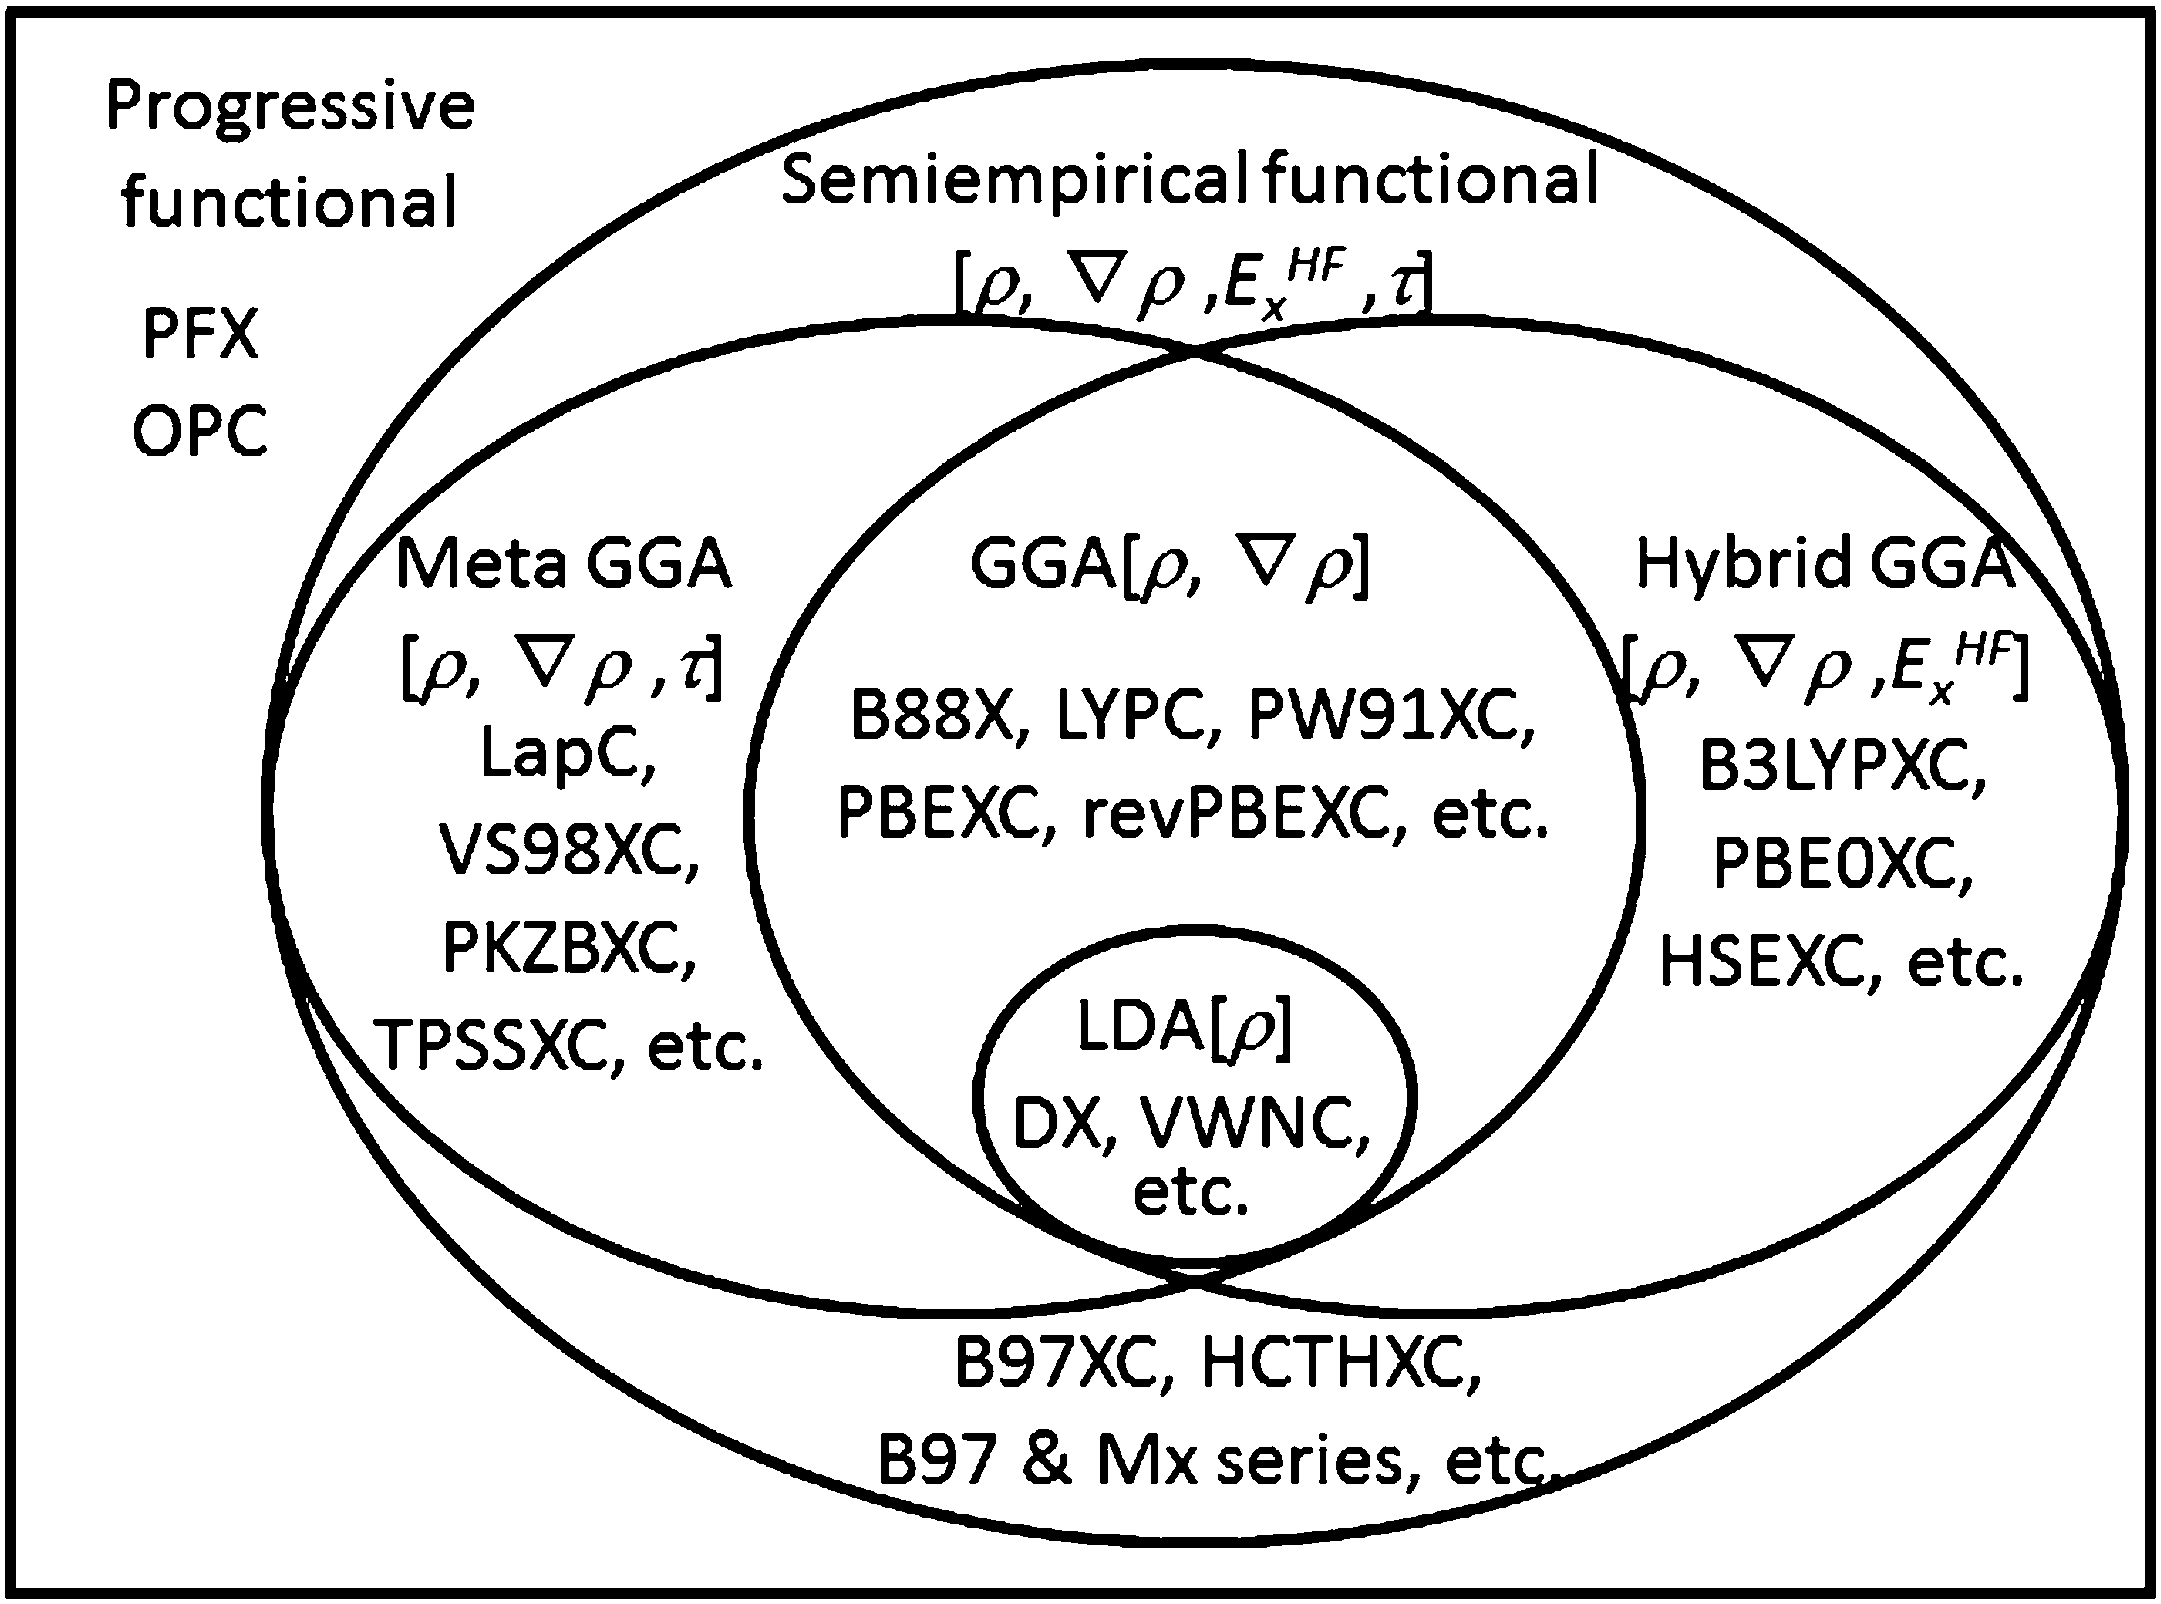
\includegraphics[width=0.5\textwidth]{functional-classification.png}
    \caption{交换-关联泛函的分类}
    \label{fig:excahnge-correlation-functional}
\end{figure}

\subsubsection{LDA近似}

当电子密度变化非常平缓时,$\grad{\rho},\laplacian{\rho}$等全部可以看成是零,此时交换关联泛函的形式是
\begin{equation}
    E_\text{XC}[\rho(\vb*{r})] = \int \dd[3]{\vb*{r}} \rho(\vb*{r}) \epsilon_\text{XC}(\rho(\vb*{r})).
\end{equation}
这就是所谓的局域密度近似:每单位的交换关联能只和该地点的电子密度有关。

首先我们尝试找一个适用于均匀自由电子气的交换关联泛函。我们取它为均匀自由电子气的基态的交换能加关联能就可以,即
\begin{equation}
    E_\text{XC}[\rho] = E_\text{X}[\rho] + E_\text{C}[\rho].
\end{equation}
自由电子气的基态就是费米面以内的每个轨道都占据了一上一下两个电子的状态,我们设共有$N$个电子,那么这些电子占据了$N/2$个不同的轨道。设这些轨道为$\{\phi_i(\vb*{r})\}$。
仅考虑库伦相互作用引入的一阶微扰,则有
\[
    E = \sum_{\sigma, \sigma'} \mel{\Psi}{
        \frac{1}{2} \int \dd[3]{\vb*{r}} \dd[3]{\vb*{r}'} \hat{\psi}^\dagger_{\sigma}(\vb*{r}) \hat{\psi}^\dagger_{\sigma'}(\vb*{r}') \frac{1}{\abs{\vb*{r} - \vb*{r}'}} \hat{\psi}_{\sigma'}(\vb*{r}') \hat{\psi}_\sigma(\vb*{r})
    }{\Psi}.
\]
这里必须完整地考虑自旋自由度的作用。可以使用Wick定理把上式展开,从而得到Hartree-Fock近似型的表达式。
请注意由于均匀电子气中没有自旋翻转,任何形如
\[
    \mel{\Psi}{\hat{\psi}_\sigma^\dagger \hat{\psi}_{\sigma'}}{\Psi}, \quad \sigma \neq \sigma'
\]
的项都是零,而
\[
    \mel{\Psi}{\hat{\psi}^\dagger_\sigma(\vb*{r}) \hat{\psi}_{\sigma}(\vb*{r}')}{\Psi} = \sum_i \phi_i^*(\vb*{r}) \phi_i(\vb*{r}'),
\]
于是最后能量修正为
\[
    E = \frac{1}{2} \int \dd[3]{\vb*{r}} \dd[3]{\vb*{r}'} \frac{1}{\abs{\vb*{r} - \vb*{r}'}} \bigg(
        \underbrace{4 \sum_{i} \abs{\phi_i(\vb*{r})}^2 \sum_{i} \abs{\phi_i(\vb*{r}')}^2}_\text{classical coulomb energy} - \underbrace{2 \sum_i \phi_i^*(\vb*{r}) \phi_i(\vb*{r}') \sum_i \phi_i^*(\vb*{r}') \phi_i(\vb*{r})}_\text{exchange energy}
    \bigg).
\]
交换能项前面的因子是$2$而不是$4$是因为自旋不同的电子之间的交换能全部抵消了。这样交换能就是
\begin{equation}
    E_\text{X} = - \int \dd[3]{\vb*{r}} \dd[3]{\vb*{r}'} \frac{1}{\abs{\vb*{r} - \vb*{r}'}} \abs{\sum_i \phi_i^*(\vb*{r}) \phi_i(\vb*{r}')}^2 . 
    \label{eq:exchange-energy-homogeneous-gas}
\end{equation}
对箱归一化的均匀电子气,有
\[
    \phi_i(\vb*{r}) = \frac{1}{\sqrt{V}} \ee^{- \ii \vb*{k}_i \cdot \vb*{r}},
\]
于是就有
\begin{equation}
    \sum_i \phi_i^*(\vb*{r}) \phi_i(\vb*{r}') = \sum_{\text{occupied $\vb*{k}$}} \frac{1}{V} \ee^{\ii \vb*{k} \cdot (\vb*{r} - \vb*{r}')} = \frac{1}{(2\pi)^3} \int_{\abs{\vb*{k}} < k_\text{F}} \dd[3]{\vb*{k}} \ee^{\ii \vb*{k} \cdot (\vb*{r} - \vb*{r}')},
    \label{eq:homogeneous-density}
\end{equation}
特别的,电子密度的一半(因为只考虑了轨道自由度)为
\[
    n(\vb*{r}) / 2 = \frac{k_\text{F}^3}{6 \pi^2}.
\]
上式代入\eqref{eq:exchange-energy-homogeneous-gas}就得到交换能的形式。
在这里我们稍微做一些推广。考虑一个非均匀的自由电子气,其非均匀性可能来自一些杂质或者特殊的相互作用,总之,每一个宏观小微观大的体积元可以看成一个用于归一化波函数的箱子,波函数定域在这个箱子里面(杂质会导致局域化)。
这样只有$\vb*{r} - \vb*{r}'$不超出一个箱子时\eqref{eq:homogeneous-density}才有明显的非零值。
每个箱子都有自己的费米动量,记作$k_\text{F}(\vb*{r})$(具体是关于$\vb*{r}$还是$\vb*{r}'$无关紧要因为两者总是在同一个箱子内)。
令
\[
    \vb*{s} = \vb*{r} - \vb*{r}', 
\]
则
\[
    \begin{aligned}
        E_\text{X} &= - \int \dd[3]{\vb*{r}} \dd[3]{\vb*{s}} \frac{1}{s} \left( \frac{1}{(2\pi)^3} \int_{\abs{\vb*{k}} < k_\text{F}} \dd[3]{\vb*{k}} \ee^{\ii \vb*{k} \cdot \vb*{s}} \right)^2 \\
        &= - \int \dd[3]{\vb*{r}} \dd[3]{\vb*{s}} \frac{1}{s} \left( \frac{3}{2} \frac{\sin t - t \cos t}{t^3} n(\vb*{r}) \right)^2 \quad (t= k_\text{F}(\vb*{r}) s) \\
        &= - 9 \pi \int \dd[3]{\vb*{r}} \int \dd{t} \frac{t}{k_\text{F}(\vb*{r})^2} n(\vb*{r})^2 \left( \frac{\sin t - t \cos t}{t^3} \right)^2 \\
        &= - \frac{3}{4} \left( \frac{3}{\pi} \right)^{1/3} \int \dd[3]{\vb*{r}} \rho(\vb*{r})^{4/3}.
    \end{aligned}
\]
这就得到了\textbf{托马斯-费米-狄拉克泛函}:
\begin{equation}
    E_\text{X}[\rho] = - \frac{3}{4} \left( \frac{3}{\pi} \right)^{1/3} \int \dd[3]{\vb*{r}} \rho(\vb*{r})^{4/3} = - 0.7386 \int \dd[3]{\vb*{r}} \rho(\vb*{r})^{4/3}
\end{equation}
对均匀或不均匀但缓变的电子气这个泛函适用。

\subsection{自洽计算}

\section{密度泛函理论的后处理}

\subsection{基态}

基态能量实际上就是能量泛函作用在基态电子密度$\rho(\vb*{r})$之后的结果。

\subsection{晶体}

对晶体的计算可以分成这么几个步骤:
\begin{enumerate}
    \item 定义晶体的几何结构,通常是通过指定一个晶胞形状,并且在晶胞内给出各个原子核的位置,这些信息——晶格矢量和晶胞内各个原子核的位置——称为\textbf{超晶胞(supercell)},通常要求超晶胞取最简单的形式,即为原胞;
    \item 
\end{enumerate}

\end{document}